\documentclass[12pt,a4paper]{article}
\usepackage[T1]{fontenc}
\usepackage[utf8]{inputenc}
\usepackage[portuguese]{babel}
\usepackage[dvipsnames]{xcolor}
\usepackage[left=2cm,right=2cm,top=2cm,bottom=2cm]{geometry}
\usepackage{amsfonts,amssymb,amsmath,enumitem,txfonts,graphicx,float,cancel}
\renewcommand{\CancelColor}{\color{red}}
\title{Trabalho de Lógica e Matemática discreta}
\author{\today}
\date{}
%%%%%%%%%%%%%%%%%%%%%%%%%%%%%%%%%% begin definitions
\DeclareMathOperator{\proj}{\bf Proj}
\setlength{\parskip}{12pt}
\newenvironment{ans}{\color{blue}\begin{quote}}{\end{quote}}
\newif \ifans
\newif \ifvf
\newcommand{\alt}{
	\ifvf
		\ifans
			\item({\sf\color{ForestGreen}V})
		\else 
			\item({\sf\color{Orange}F}) 
		\fi
	\else
		\ifans
			\item({\sf\color{Cyan}X})
		\else 
			\item({\sf\phantom{X}}) 
		\fi	
	\fi	
	\ansfalse
	\vffalse
}
\def\X{\anstrue}
\def\V{\vftrue\anstrue}
\def\F{\vftrue}
%%%%%%%%%%%%%%%%%%%%%%%%%%%%%%%%%% end definitions
\begin{document}
\maketitle










\begin{enumerate}
%%%%%%%%%% 1
\item Em um colégio há equipes de vôlei, futebol e basquete. Neste semestre um fato pitoresco acontecerá: quando tiver treino de basquete não terá treino de vôlei. Uma forma equivalente de se dizer esse fato pitoresco é
	\begin{enumerate}
	\alt Quando não tiver treino de basquete, terá treino de vôlei.
	\X\alt Quando tiver treino de vôlei, não terá treino de basquete.
	\alt Quando não tiver treino de vôlei, terá treino de basquete.
	\alt Quando tiver treino de vôlei, poderá ter treino de basquete.
	\alt Nenhuma das alternativas anteriores está correta.
	\end{enumerate}
	
	\begin{ans}
	Quando temos uma proposição unidirecional, do tipo $A\Rightarrow B$ (se A, então B), uma proposição equivalente, chamada de contrapositiva, é $(\sim B)\Rightarrow (\sim A)$ (se não B, então não A). Sabendo disso, vamos relacionar à proposição da questão:

\begin{itemize}
	\item $A$: há treino de basquete
	\item $B$: não há treino vôlei.	
	\item[$\bigstar$] $A\Rightarrow B$: se há treino de basquete, então não há treino de vôlei.	
	\item[*] $(\sim A)$: não há treino de basquete
	\item[*] $(\sim B)$: há treino de vôlei.
	\item[$\bigstar$] $(\sim B)\Rightarrow(\sim A)$: se há treino de vôlei, então não há treino de basquete.
	\end{itemize}
	As duas proposições em $\bigstar$ são equivalentes.
	\end{ans}
	
	
	
	
	
	
	
	
%%%%%%%%%% 2
\item Qual o termo independente do binômio
\[
\left(x^3+\frac{1}{x}\right)^{12}	
\]
	\begin{enumerate}
	\alt 120
	\alt 180
	\X\alt 220
	\alt 792
	\alt 924
	\end{enumerate}
	
	\begin{ans}
	Os binômios to tipo $(a+b)$ quando elevados a uma certa potência $n$ podem ser escritos como
	\[
	(a+b)^n = \binom{n}{0}a^0b^n+\binom{n}{1}a^1b^{n-1}+\binom{n}{2}a^2b^{n-2}+...+\binom{n}{n-1}a^{n-1}b^1+\binom{n}{n}a^nb^0
	\]
	ou escrito mais concisamente como (note que a soma dos expoentes de $a$ e $b$ é sempre $n$)
	\[\tag{1}\label{eq}
	(a+b)^n = \sum_{k=0}^{n}\binom{n}{k}\;a^kb^{n-k}.
	\]
	Em que $\binom{n}{p}$ representa o número de combinações de $n$ itens tomados $p$ a $p$, dados pela fórmula
	\[\tag{2}\label{eq2}
	\binom{n}{p}=\frac{n!}{p!(n-p)!}.
	\]
	Uma forma simples de calcular os binômios $\binom{n}{p}$ é usando o Triângulo de Pascal:
	\[
	\def\r{\color{red}}
	\def\s{\color{cyan}}
	\begin{array}{c|cccccc}
	& 0 & 1 & 2 & 3 & 4 & p\\
	\hline
	0 & 1\\
	1 & \r 1 &\r 1\\
	2 & 1 &\r 2 & 1\\
	3 & 1 & \s 3 & \s 3 & 1\\
	4 & 1 & 4 & \s 6 & 4 & 1\\
	n & \vdots & \vdots & \vdots & \vdots & \vdots & \ddots
	\end{array}
	\]
	O Triângulo de Pascal tem a primeira coluna e a diagonal de 1's,
	em que cada elemento abaixo da diagonal é a soma entre dois elementos da linha de cima, o elemento imediatamente acima e o à esquerda deste, conforme indicado pelas cores no exemplo acima.
	
	Por exemplo, consultando o Triângulo de Pascal acima, podemos escrever facilmente os seguintes binômios
	\[
	\def\r{\color{red}}
	\def\s{\color{green}}
	(a+b)^3 = {\r 1}a^{\s 3}b^{\s 0}+{\r 3}a^{\s 2}b^{\s 1}+{\r 3}a^{\s 1}b^{\s 2}+{\r 1}a^{\s 0}b^{\s 3}=a^3+3a^2b+3ab^2+b^3,
	\]
	\[
	\def\r{\color{red}}
	(a+b)^4 = {\r 1}a^4+{\r 4}a^3b+{\r 6}a^2b^2+{\r 4}ab^3+{\r 1}b^4
	.\]
	
	Para o problema dado, precisamos verificar qual é o expoente $p$ de modo que (veja a Equação \eqref{eq})
	\[
	(x^3)^p\left(\frac{1}{x}\right)^{12-p}=x^{3p}\left(\frac{1}{x^{12-p}}\right)=\frac{x^{3p}}{x^{12-p}}=\text{constante}.\quad \color{cyan}(a^pb^{n-p})
	\]
	Precisamos que $p$ seja um inteiro que faça com que numerador e denominador sejam iguais, pois assim a fração resultaria em $1$. Isso é fácil, basta resolver a equação 
	\[
	x^{3p}=x^{12-p} \iff
	3p=12-p\iff 4p=12\iff p=3.
	\]
	Agora, usando as Equações \eqref{eq} e \eqref{eq2}, podemos descobrir qual é o coeficiente desejado:
\[
\binom{12}{3}\;(x^3)^3\left(\frac{1}{x}\right)^{12-3}=\binom{12}{3}\;x^9\frac{1}{x^9}=\binom{12}{3} \stackrel{\text{Eq.}\eqref{eq2}}{=} \frac{12!}{3!(12-3)!}=\frac{12.11.10.9!}{9!6}=2.11.10=220
\]	

	\end{ans}






%%%%%%%%%% 3
\item Um professor pretende realizar uma atividade com 6 alunos. Estes alunos ficarão em círculo. Sabendo-se que André e Maria não poderão ficar juntos na atividade, porque conversam muito, de quantas formas o professor poderá organizar os 6 alunos?
	\begin{enumerate}
	\alt 120
	\X\alt 72
	\alt 48
	\alt 24
	\alt 12
	\end{enumerate}
	
	\begin{ans}
	Vamos fixar Maria (M) em uma posição, escolher uma posição para André (A) e contar as possibilidades para as demais posições:
	\[
	\begin{aligned}
	\frac{M}{}\;\;
	\frac{4}{\;\xcancel{A}\;}\;\;
	\frac{A}{\quad}\;\;
	\frac{3}{\quad}{}\;\;
	\frac{2}{\quad}{}\;\;
	\frac{1}{\;\xcancel{A}\;}
	\\\\
	\frac{M}{}\;\;
	\frac{4}{\;\xcancel{A}\;}\;\;
	\frac{3}{\quad}{}\;\;
	\frac{A}{\quad}\;\;
	\frac{2}{\quad}{}\;\;
	\frac{1}{\;\xcancel{A}\;}
	\\\\
	\frac{M}{}\;\;
	\frac{4}{\;\xcancel{A}\;}\;\;
	\frac{3}{\quad}{}\;\;
	\frac{2}{\quad}\;\;
	\frac{A}{\quad}{}\;\;
	\frac{1}{\;\xcancel{A}\;}
	\end{aligned}
	\]
	Qualquer rotação dessas disposições formará o mesmo círculo, algo como: $M P A R S T = P A R S T M = A R S T M P=RSTMPA$, etc. Assim, todas as possibilidades já estão contabilizadas, bastando multiplicar e somar, um total de $3 \times 24=72$.
	\end{ans}
	




%%%%%%%%%% 4
\item Um palácio tem 5 portas. De quantas maneiras se pode abrir este palácio?
	\begin{enumerate}
	\alt 5
	\alt 15
	\alt 18
	\X\alt 31
	\alt 32
	\end{enumerate}
	
	\begin{ans}
	A questão se resume a combinar quais portas serão abertas. Do total de 5 portas, podemos escolher uma porta para abrir, duas portas, 3, 4 ou as 5 portas. As combinações são, respectivamente, $\binom{5}{k}$, com $k=1,2,3,4,5$. Note que não usamos o caso $k=0$, pois seria o caso em que nenhuma porta seria aberta.	
	
	Para responder à pergunta, complete o Triângulo de Pascal até a linha $n=5$ e então faça a soma das possibilidades. O total será 31.
	\end{ans}





%%%%%%%%%% 5
\item Em uma prova de tiro ao alvo, Marcelo tem probabilidade de acertar o alvo de $\frac{2}{7}$ e a probabilidade de Antônio acertar o mesmo alvo é de $\frac{2}{5}$. Qual é a probabilidade de pelo menos um dos dois acertar o alvo, considerando que ambos atiram ao mesmo tempo?
	
	\begin{enumerate}
	\alt $\frac{4}{35}$
	\alt $\frac{8}{35}$
	\alt $\frac{16}{35}$
	\X\alt $\frac{20}{35}$
	\alt $\frac{32}{35}$
	\end{enumerate}
	
	\begin{ans}
	Marcelo acerta e Antônio erra com probabilidade $\frac{2}{7}\cdot \frac{3}{5}=\frac{6}{35}$, Marcelo erra e Antônio acerta com probabilidade $\frac{5}{7}\cdot \frac{2}{5}=\frac{10}{35}$. Ambos acertam com probabilidade $\frac{2}{7}\cdot \frac{2}{5}=\frac{4}{35}$. Somando tudo, temos $\frac{20}{35}$ de probabilidade de pelo menos um deles acertar.
	\end{ans}








%%%%%%%%%% 6
\item Uma empresa faz salgadinhos para festas. Os salgadinhos disponíveis para encomendas são: coxinha, bolinha de queijo, quibe, empadinha e pastelzinho. Em cada encomenda, o cliente poderá escolher até 3 tipos de salgadinhos. Observe que não há a necessidade de pedir salgadinhos distintos. Por exemplo, pedir duas porções de coxinha e uma porção de pastelzinho. De quantas formas se pode fazer pedidos para essa empresa?	
	\begin{enumerate}
	\alt 5
	\alt 10
	\alt 20
	\alt 30
	\X\alt 35
	\end{enumerate}
	
	
	\begin{ans}
	Suponha que o cliente peça 1 porção apenas. Então temos 5 possibilidades:
	\[
	\frac{5.}{\quad}
	\]
	 Suponha que peça 2 porções, em que os itens são diferentes do tipo $(a,b)$:
	\[
	\frac{5}{\quad} \;\;\frac{4.}{\quad}
	\]
	Temos um total de 20 possibilidades. No entanto, quando fazemos um arranjo simples dessa forma, estamos dizendo que $(a,b)\neq(b,a)$, mas são o mesmo pedido! Precisamos então descontar esses casos que contamos demasiadamente, dividindo o resultado pelo número de permutações que é $2!=2$. Portanto, temos $20/2=10$ possibilidades, nas quais os itens $(a,b)=(b,a)$ são considerados iguais. Agora, como os pedidos podem ser repetidos, precisamos contá-los (os casos do tipo $(a,a)$, que são um total de 5). O total de possibilidades para pedir 2 porções é 15.
	
	Suponha que o cliente peça três porções diferentes, e analogamente ao caso anterior, 
	\[
	\frac{5}{\quad} \;\;\frac{4}{\quad}\;\;\frac{3.}{\quad}
	\]
	Daí temos um total de $60$ possibilidades. Mas estamos contando como sendo diferentes os pedidos da forma $(a,b,c)\neq(a,c,b)\neq(b,c,a)$, etc. Para descontar os itens contados indevidamente, precisamos dividir pelo total de suas permutações, que é $3!=6$. Assim, o resultado é $60/6=10$. Mas ainda não contamos os casos do tipo $(a,a,a)$, que são 5. Por fim, temos 15 possibilidades.
	
	A resposta final é a soma dos 3 casos, 35.
	
	\end{ans}









%%%%%%%%%% 7
\item Considere uma urna com bolas numeradas de 1 a 50. Qual a probabilidade de se tirar um número que seja múltiplo de 2, 3 ou 5 em um único sorteio?
	\begin{enumerate}
	\alt 32\%
	\alt 48\%
	\alt 56\%
	\alt 64\%
	\X\alt 72\%
	\end{enumerate}
	
	\begin{ans} 
	Vamos contar quantos números são múltiplos de 2, 3 e 5. Uma forma rápida de fazer isso, já que a lista começa em 1 e vai até 50, é pegar a função ``chão'' $f(k)=\lfloor \frac{50}{k}\rfloor$, $k=2,3,5$, definida como sendo o arredondamento para baixo para o inteiro mais próximo (ou dito de outra forma, o maior inteiro menor ou igual a $50/k$). Estamos dividindo 50 por 2, 3, 5, e pegando apenas a parte inteira. 
	Isso nos dá 
	\[
	f(2)=\lfloor \frac{50}{2}\rfloor=\lfloor 25\rfloor=25,
	\]
	\[
	f(3)=\lfloor \frac{50}{3}\rfloor=\lfloor 16.\bar 6\rfloor=16
	\]
	\[
	f(5)=\lfloor \frac{50}{5}\rfloor=\lfloor 10\rfloor=10.
	\]
	
	Dentre os 25 múltiplos de 2, há os que são múltiplos de 3, e também os múltiplos de 5 (no final das contas, são múltiplos de 6 e 10). Vamos contá-los:
	 \[
	 f(6)=\lfloor \frac{50}{6}\rfloor=\lfloor 8.\bar 3\rfloor=8,
	 \]
	 \[
	 f(10)=\lfloor \frac{50}{10}\rfloor=5.
	 \] Também temos os que são múltiplos de 3 e 5, ou seja, múltiplos de 15:
	 \[
	 f(15)=\lfloor \frac{50}{15}\rfloor=\lfloor 3.\bar 3\rfloor=3.
	 \]
	 Por fim, os que são múltiplos de 2, 3 e 5, ou seja, múltiplos de 30:
	 \[
	 f(30)=\lfloor \frac{50}{30}\rfloor=\lfloor 1.\bar 6\rfloor=1.
	 \]
	 Podemos colocar essas informações num diagrama de Venn, conforme a Figura \ref{venn}. 
	 
	Agora, basta contar, o que dá um total de 36 dentre 50 valores, ou seja, $36/50=0.72=72\%$.
	 \begin{figure}[h!tb]\centering
	 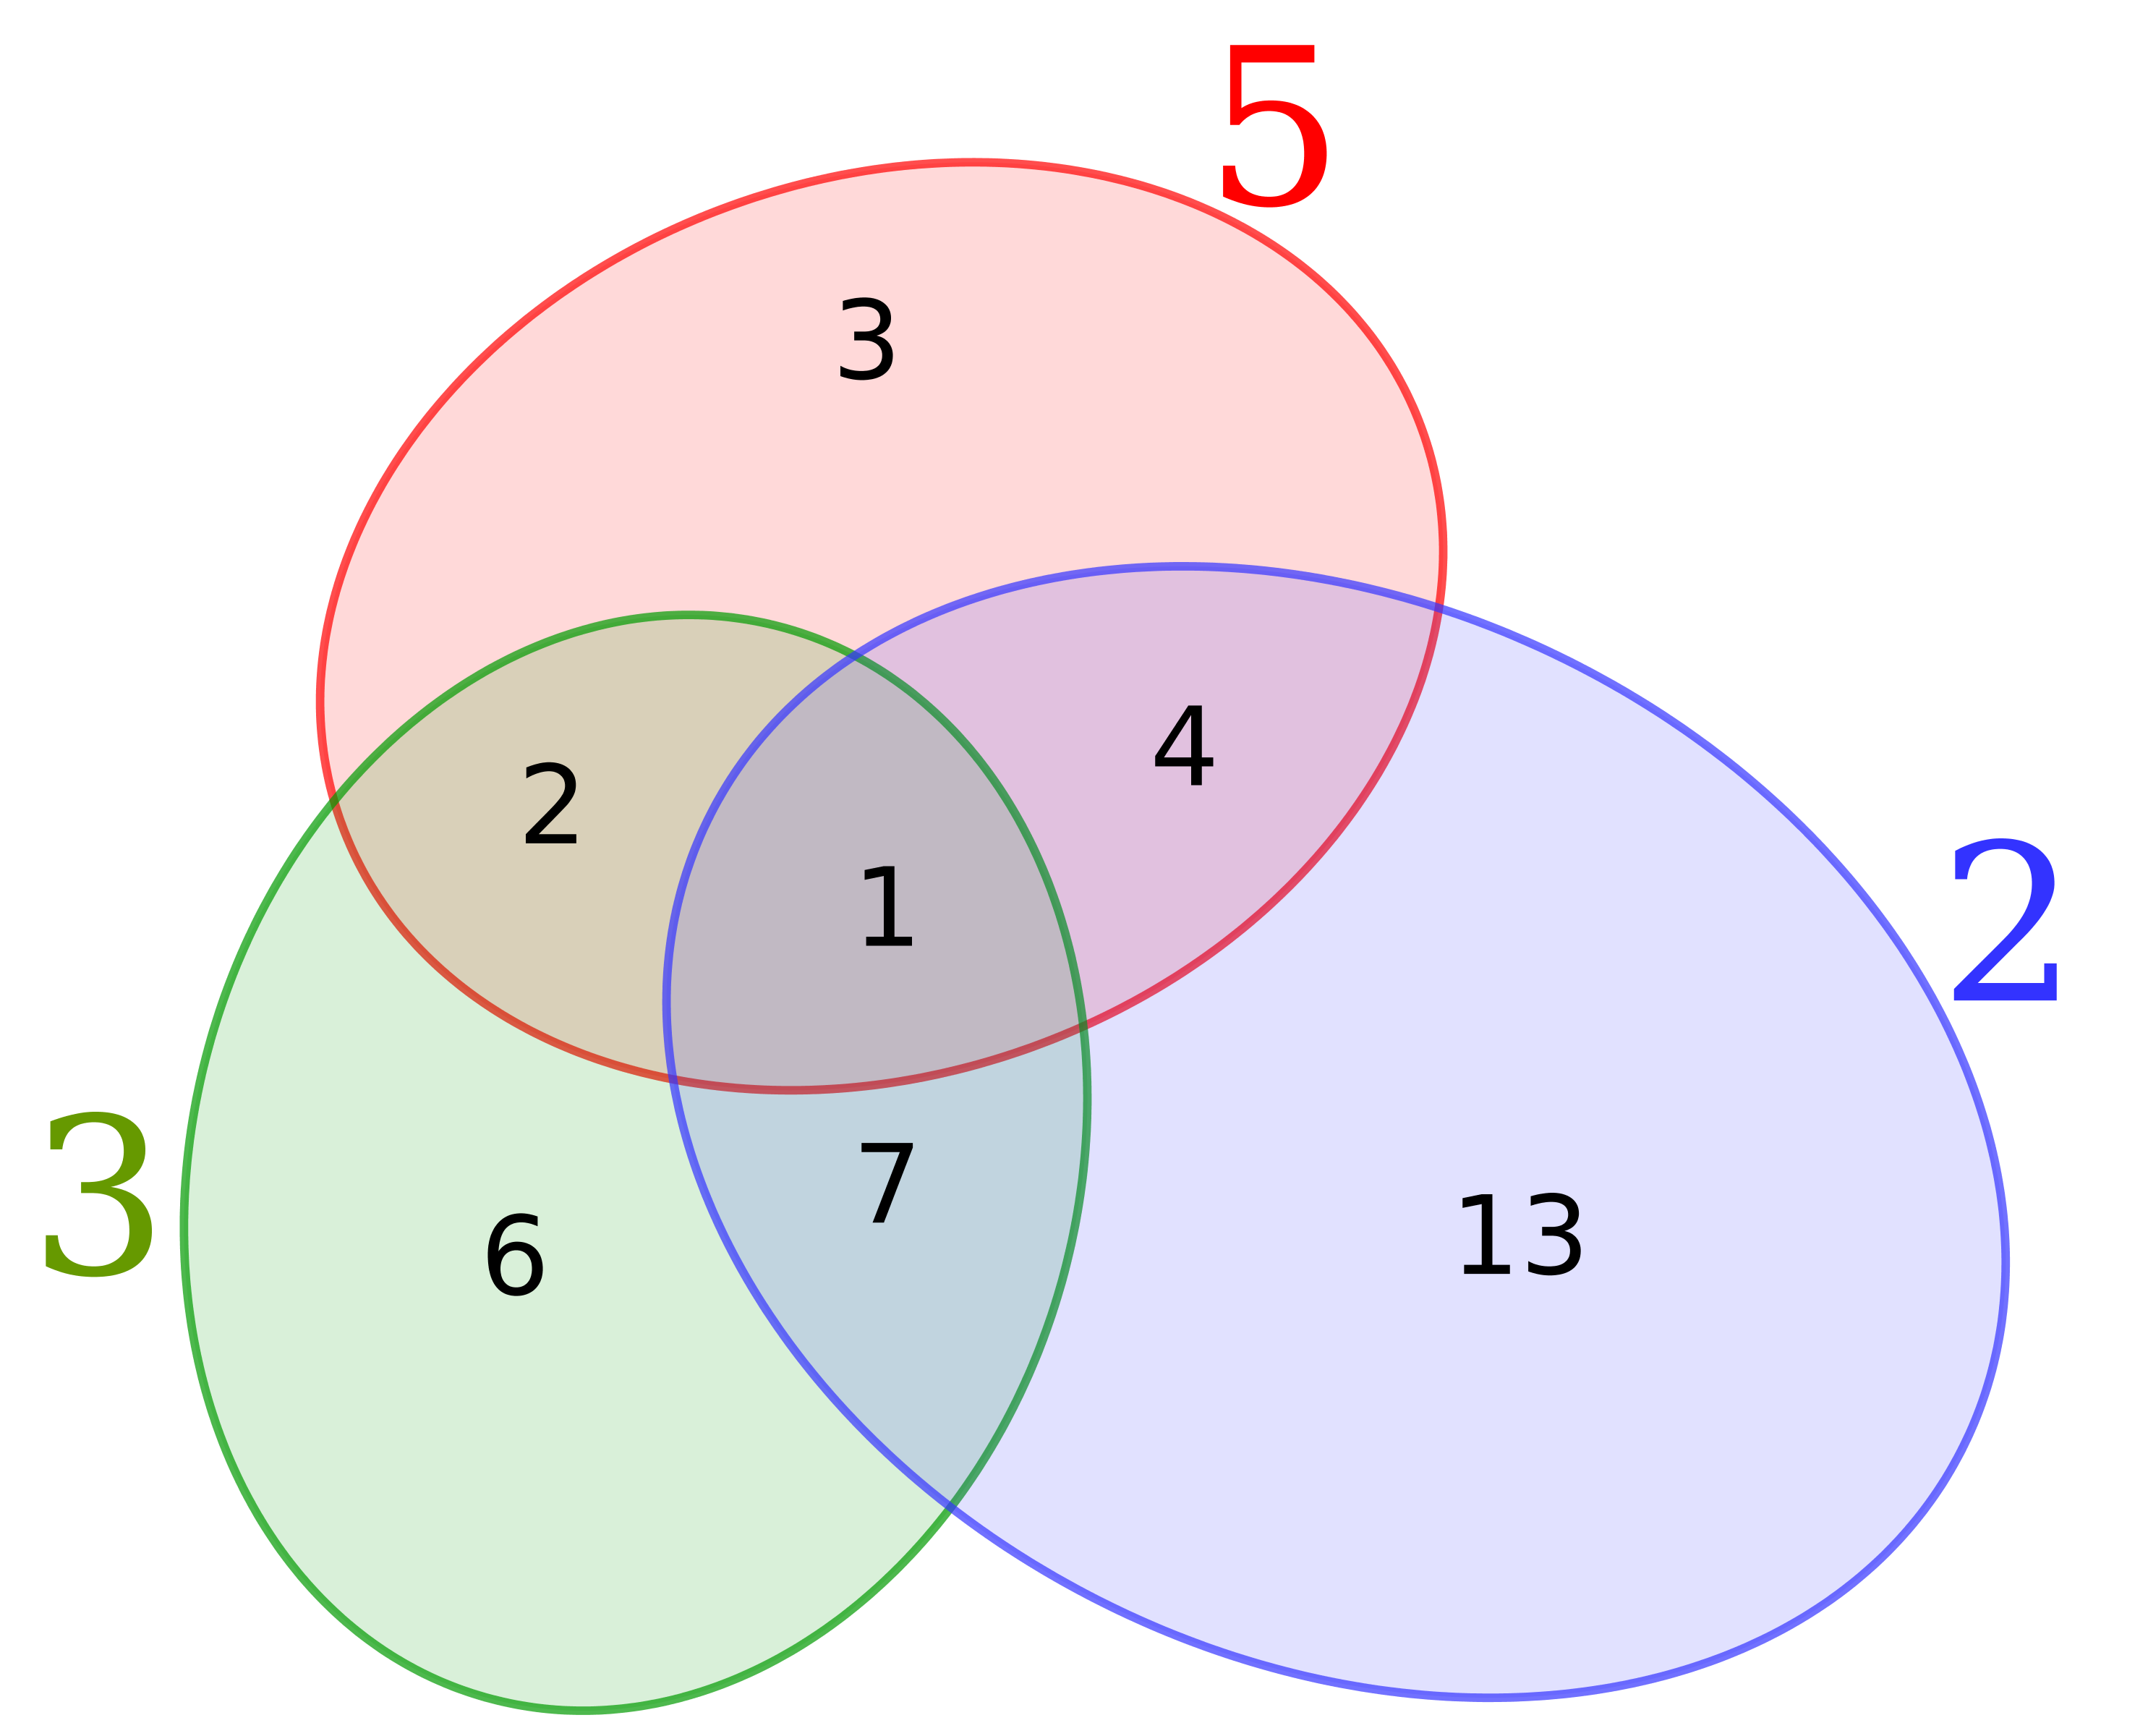
\includegraphics[height=0.2\textheight]{venn}
	 \caption{A quantidade de múltiplos dentre 1 e 50.}\label{venn}
	 \end{figure}
	\end{ans}



%%%%%%%%%% 8
\item Na empresa X os funcionários têm uma senha para acessar os sistemas da empresa. Cada senha é formada por um número par de 4 algarismos. Quantas senhas são possíveis formar com os algarismos de 0 a 9 inclusive?
	\begin{enumerate}
	\F\alt 2296
	\F\alt 2846
	\F\alt 3024
	\F\alt 4048
	\F\alt 5264
	\end{enumerate}
	
	\begin{ans}
	Precisamos preencher as lacunas com algarismos: $\_\_\;\;\_\_\;\;\_\_\;\;\_\_ $. Em cada lacuna, colocamos as possibilidades:
	$\underline{9}\;\;\underline{10}\;\;\underline{10}\;\;\underline{5}$ com um total de 4500 possibilidades (basta multiplicar). 9 porque não podemos incluir o zero no primeiro dígito. Os dois 10 porque podemos incluir qualquer dígito, sem restrições. 5 porque a senha precisa ser um número par, e portanto precisa terminar em 0, 2, 4, 6 ou 8 (5 possibilidades).
	
	\end{ans}
	




%%%%%%%%%% 9
\item Considere um conjunto $A$ com $n$ elementos. Define-se uma partição de $A$ como uma família de conjuntos $A_1$, $A_2$, ..., $A_k$ todos não vazios de modo que $A_1\cup A_2\cup...\cup A_k=A$ e os conjuntos $A_i$ são todos disjuntos, ou seja, $A_i\cap A_j=\emptyset$ para todo $i\neq j$. Dizemos também que $A$ foi particionado em $A_1$, ..., $A_k$. Diante disso, assinale a alternativa correta
	
	\begin{enumerate}
	\alt O número de conjuntos da  partição $A_1,...,A_k$ é $2^n$.
	\alt O número de conjuntos da  partição $A_1,...,A_k$ é $2^n-2$ pois não são considerados nem o conjunto vazio, nem o próprio $A$.
	\X\alt Há um número finito de conjuntos que particionam o conjunto $A$ e o número máximo de uma família de conjuntos $A_1,...,A_k$ que particiona o conjunto $A$  é igual a $n$.
	\alt Há infinitas formas de se particionar o conjunto $A$.
	\alt As alternativas (b) e (d) estão corretas.
	\end{enumerate}
	
	\begin{ans}
	\begin{enumerate}
	\item Contraexemplo: seja $A=\{a,b,c,d,e,f\}$. Temos $n=6$ e uma possível partição é $\{c\}\cup\{d,f\}\cup\{a,b,e\}$, um total de 3 conjuntos, o que obviamente não é $2^6=64$.
	\item O mesmo contraexemplo acima serve para esta.
	\item A partição unitária é aquela em que cada subconjunto contém apenas um elemento cada um. No exemplo de (a), a partição unitária é $\{a\}\cup\{c\}\cup\{b\}\cup\{d\}\cup\{f\}\cup\{e\}$ com um total de 6 conjuntos, o mesmo valor de  $n$. Percebe-se que $n$ é o maior número de conjuntos possível para uma partição. Como $n$ é finito, há um número finito de conjuntos que particionam $A$.
	\item falsa pela explicação em (c).
	\end{enumerate}
	\end{ans}
	

%%%%%%%%%% 10	
\item Com relação à demonstração por absurdo e a demonstração por indução finita é correto afirmar que
	\begin{enumerate}
	\alt A demonstração por absurdo e a demonstração por indução finita 	consistem em uma mesma forma de demonstrar teoremas e outros resultados em matemática.
	\alt Na demonstração por absurdo, considera-se como verdadeiro uma hipótese falsa e se chegar  em um resultado verdadeiro significa que a demonstração foi realizada com sucesso.
	\alt Não há necessidade da hipótese de indução em algumas situações no método de demonstração por indução finita.
	\alt As alternativas (b) e (c) estão corretas.
	\X\alt Nenhuma das alternativas anteriores está correta.
	\end{enumerate}
	
	\begin{ans}
	\begin{enumerate}
	\item são demonstrações diferentes.
	\item uma hipótese falsa é considerada como verdadeira, e precisamos chegar a um resultado falso para refutar a hipótese falsa assumida.
	\item a hipótese de indução é o cerne da demonstração, pois é o fato que permite ligar um caso $n$ ao caso $n+1$.
	\end{enumerate}
	
	\end{ans}
	
	
\end{enumerate}

\end{document}